\section{Stub Finding in the CBC3}
The CBC3 is the first version of the 2S module read-out ASIC to include the full logic circuitry required for stub finding. A 2S module prototype, constructed with two sensors separated by ${1.8}$\mm and a double-sided rigid hybrid with two bump-bonded CBC3 chips, was used to test the logic using the 120 GeV proton beam at the Fermilab Test Beam Facility. \Cref{fig:stubs} shows the stub-finding efficiency for different correlation windows : a programmable on-chip register which defines the maximum distance (in strips) between clusters on a valid stub. The measurement shows that the stub is high (${>95\%}$) and that the cut-off is in agreement with that expected for the given sensor strip pitch and spacing.

% This exploits the relationship between a proton's angle of incidence ($\theta$) on the module and the longitudinal seperation (${\delta x}$) between the corresponding hits in the two sensors ; on a module at radius $R$ is exploited to emulate the effect of a $3.8$\,\tesla\, magnetic field on charged particles  
% \begin{equation}
% p_T = \frac{0.57R}{\sin(\theta)}\approx0.57R\sqrt{1 + (\frac{d}{\Delta{x}})^2}
% \end{equation}

\begin{figure}[!htbp]
\centering
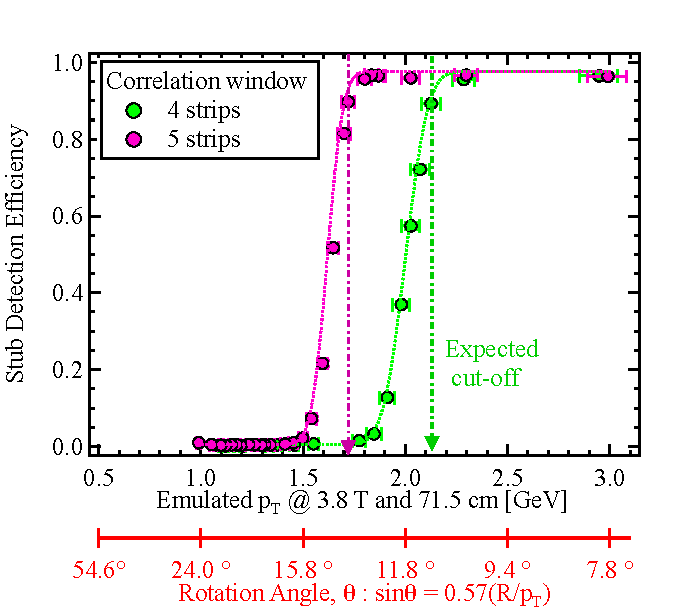
\includegraphics[width=0.9\linewidth]{Figures/StubScan.pdf}
\vspace*{-2mm}
\caption{Stub detection efficiency as a function of emulated transverse momemtum ${p_T}$; the expected ${p_T}$ cut-off estimated from the strip pitch (${90}$\microns) and the sensor spacing ${1.8}$\mm is also shown. The prototype was rotated with respect to the beam-axis to mimic the effect of charged particles bending in a magnetic field at a radius $R$ of ${71.5}$\cm.}
\label{fig:stubs}
\end{figure}
